\documentclass[a4paper,11pt]{article}

\usepackage{amsmath,amssymb,amsthm,amsopn,natbib,anysize}
\marginsize{2.5cm}{2.5cm}{2.5cm}{2.5cm}


\renewcommand{\today}{\begingroup
\number \day\space  \ifcase \month \or January\or February\or March\or 
April\or May\or June\or July\or August\or September\or October\or 
November\or December\fi 
\space  \number \year \endgroup}

\renewcommand{\vec}[1]{\boldsymbol{#1}}
\newcommand{\gvec}[1]{\boldsymbol{#1}}
\newcommand{\mat}[1]{\mathbf{#1}}
\newcommand{\gmat}[1]{\boldsymbol{#1}}
\newcommand{\bmat}[4]{\begin{bmatrix} #1 & #2 \\ #3 & #4\end{bmatrix}}
\newcommand{\argmin}[1]{\underset{#1}{\mathrm{argmin}} \ }
\newcommand{\argmax}[1]{\underset{#1}{\mathrm{argmax}} \ }
\newcommand{\indi}[1]{\boldsymbol{1} \lbrace #1 \rbrace}

\def\jneqi{\substack{j=1 \\ j\neq i}}
\def\kneqj{\substack{k=1 \\ k\neq j}}
\def\HH{\mat{H}}
\def\G{\mat{G}}
\def\ks{\texttt{ks}}
\def\sm{\texttt{sm}}
\def\KernSmooth{\texttt{KernSmooth}}
\def\MSE{\mathrm{MSE}}
\def\MISE{\mathrm{MISE}}
\def\AMSE{\mathrm{AMSE}}
\def\AMISE{\mathrm{AMISE}}
\def\SAMSE{\mathrm{SAMSE}}
\def\SCV{\mathrm{SCV}}
\def\PI{\mathrm{PI}}
\def\NR{\mathrm{NR}}
\def\BCV{\mathrm{BCV}}
\def\LSCV{\mathrm{LSCV}}
\def\vecr{\vec{r}}
\def\vecx{\vec{x}}
\def\vecy{\vec{y}}
\def\vecX{\vec{X}}
\def\intr2{\int_{\boldsymbol{\mathbb{R}}^2}}

\DeclareMathOperator{\E}{\boldsymbol{\mathbb{E}}}
\DeclareMathOperator{\Var}{Var}
\DeclareMathOperator{\Cov}{Cov}
\DeclareMathOperator{\Prob}{\boldsymbol{\mathbb{P}}}
\DeclareMathOperator{\given}{\vert}
\DeclareMathOperator{\Bias}{Bias}
\DeclareMathOperator{\VEC}{vec}
\DeclareMathOperator{\VECH}{vech}
\DeclareMathOperator{\tr}{tr}
\DeclareMathOperator{\dg}{dg}
\DeclareMathOperator{\diag}{diag}

%\VignetteIndexEntry{ks} 
%\SweaveOpts{}

\title{Using ks for bivariate kernel density estimation}
\author{Tarn Duong \\Department of Statistics, University of New South Wales\\ Sydney Australia}


\usepackage{/usr/lib/R/share/texmf/Sweave}
\begin{document}

\maketitle

\section{Introduction}
  
Kernel density estimation has become a popular tool for visualising 
the distribution of data. See \citet*{simonoff96}, for example, for an overview. 
When multivariate kernel density estimation is considered it is usually
in the constrained context with diagonal bandwidth matrices 
e.g. the \texttt{R} packages \texttt{sm} and \texttt{KernSmooth}.  
We introduce a new package \texttt{ks} for 
kernel smoothing with unconstrained bandwidth
matrices. Currently kernel density estimation and kernel discriminant
analysis for 1- to 6-dimensional data  are available.  
This vignette focuses on kernel density estimation for the 2-dimensional case.

\section{Kernel density estimation}

For a bivariate sample $\vecX_1, \vecX_2, \ldots, \vecX_n$ drawn from a density $f$, 
the kernel density estimate is 
\begin{equation}
\hat{f} (\vecx; \HH) = n^{-1}\sum_{i=1}^n K_{\HH} ( \vecx - \vec{X}_i)
\label{eq:kde}
\end{equation}
where $\vecx = (x_1, x_2)^T$ and $\vec{X}_i = (X_{i1}, X_{i2})^T, i = 1, 2,  
\ldots, n$.  
Here 
$K(\vecx)$ is the bivariate kernel (which we assume to be a probability density 
function); $\HH = \begin{bmatrix}h_1^2 & h_{12} \\ h_{12}& h_2^2 \end{bmatrix}$ 
is the bandwidth matrix which is symmetric and positive-definite; 
and $K_{\HH}(\vecx) = |\HH|^{-1/2} 
K( \HH^{-1/2} \vecx)$. 
The choice of $K$ is not crucial -- we take 
$K(\vecx) = (2\pi)^{-1} \exp(-\tfrac{1}{2} \vecx^T \vecx)$ the standard normal
throughout.  
On the other hand, the choice of $\HH$ \emph{is} crucial in determining 
the performance of $\hat f$. 

We measure the performance of $\hat f$ (in common with the 
majority of researchers in this field) 
using the Mean Integrated Squared Error (MISE) criterion, 
$$
\MISE \, (\HH)
= \E \int_{\mathbb{R}^2} [ \hat{f}(\vecx; \HH) - f(\vecx) ] ^2
\ d \vecx.
$$
Our aim in bandwidth selection is to estimate
$$\HH_\MISE = \underset{\HH}{\mathrm{argmin}} \
\MISE \,(\HH),
$$
over the space of all symmetric, positive definite $2 \times 2$ 
matrices. It is
well known that the optimal bandwidth $\HH_{\MISE}$ does not have a closed form. 
To make progress it is usual to employ an asymptotic approximation, known 
as the AMISE (Asymptotic MISE): 
\begin{equation}
\AMISE \,(\HH) = (4\pi)^{-1}  n^{-1}  |\HH| ^{-1/2}
 + \tfrac{1}{4} (\VECH^T \HH) \gmat{\Psi}_4(\VECH \, \HH)
\label{eq:amise}
\end{equation}
where  vech is the vector half 
operator i.e.
$$\VECH \HH = \VECH \begin{bmatrix} h_1^2  & h_{12} \\ h_{12} & h_2^2 \end{bmatrix}
= \begin{bmatrix} h_1^2 \\ h_{12} \\ h_2^2 \end{bmatrix}.$$ 
We can show that 
\begin{equation}
\gmat{\Psi}_4 =
\begin{bmatrix}\psi_{40} & 2\psi_{31} & \psi_{22} \\
2\psi_{31} & 4\psi_{22} & 2\psi_{13} \\
\psi_{22} & 2\psi_{13} & \psi_{04}
\end{bmatrix}
\label{Psi}
\end{equation}
where the integrated density derivative functional is
$$
\psi_{r_1, r_2} = \int_{\mathbb{R}^2} 
f^{(r_1, r_2)} (\vecx) f(\vecx)\ d \vecx
$$
and the partial derivatives of $f$ are $$
f^{(r_1, r_2)} (\vecx) =  \frac{\partial^{4}} 
{\partial^{r_1}_{x_1} \partial^{r_2}_{x_2}} f(\vecx). 
$$
(Note that the subscript 4 on $\gmat{\Psi}$ relates to the order of the 
derivatives involved).

We make use of the tractability of AMISE by seeking
$$
\HH_\AMISE = \underset{\HH}{\mathrm{argmin}} \ \AMISE \,
(\HH)
$$
rather than $\HH_\MISE$. 
For the next step we estimate the AMISE. The
minimiser of the $\widehat{\AMISE}$ is then a data-driven bandwidth selector
i.e. \begin{equation} 
\hat{\HH} = \underset{\HH}{\mathrm{argmin}} \ \widehat{\AMISE} \,
(\HH).
\end{equation}


\section{Plug-in bandwidth selectors}
\label{sec:plugin}

The most well-known univariate plug-in selector is due to
\citet*{sheather91}.
Plug-in selectors require pilot estimates of the
$\psi_{r_, r_2}$ functionals which comprise 
$\hat{\gmat{\Psi}}_4$. This in turn produces an estimate of the AMISE
\begin{equation}
\PI (\HH) = n^{-1} |\HH| ^{-1/2}
R(K) + \tfrac{1}{4}  (\VECH^T \HH) \hat{\gmat{\Psi}}_4(\VECH \HH)
\label{eq:api}
\end{equation}
that can be numerically minimised to give the plug-in bandwidth matrix, 
$\hat{\HH}_\PI$.  
To compute $\hat{\gmat{\Psi}}_4$ we need to use a helper or `pilot' bandwidth
matrix $\G$. Like $\HH$, we need to choose a sensible value for $\G$.  
If we note that 
$\psi_{r_1, r_2}= \E f^{(r_1, r_2)}(\vec{X})$ where $\vecX \sim f$,
then a natural estimator of $\psi_{r_1, r_2}$ is
\begin{equation}
\hat{\psi}_{r_1, r_2} (\G) = n^{-1}
\sum_{i=1}^n \hat{f}^{(r_1, r_2)} (\vec{X}_i; \G) =
n^{-2}\sum_{i=1}^{n}\sum_{j=1}^{n} K^{(r_1, r_2)}_{\G} (\vec{X}_i -
\vec{X}_j).
\label{psir} 
\end{equation}


\subsection{AMSE pilot bandwidth selectors}

We consider pilot bandwidth matrices of the form 
$\G = g^2 \mat{I}$. It may appear that we are contradicting
ourselves since we advocate using unconstrained matrices for $\HH$.
It turns out that a restricted form on $\G$ has less effect on the
performance of $\hat{f}$ than a restricted form on $\HH$. We can 
reduce the effect of the restricted form of $\G$ by using
an appropriate pre-transformation 
(we return to this topic in Section \ref{sec:pre}).

The AMSE-optimal pilot bandwidths (i.e. optimal for the Asymptotic
Mean Squared Error) are 
(a) if both $r_1$ and $r_2$ are even then
\begin{equation}
\label{eq:gamse_even} g_{r_1, r_2, \AMSE} = \bigg[ \frac{A_{r_1, r_2}}{n} 
\bigg]^{1/8}
\end{equation}
and (b) if at least one of $r_1$ and $r_2$ is odd then 
\begin{equation}
\label{eq:gamse_odd} g_{r_1, r_2, \AMSE} = \bigg[ \frac{B_{r_1, r_2}}{n} 
\bigg]^{1/7}.
\end{equation}
See \citet*{wand94} for explicit expressions for $A_{r_1, r_2}$ and
$B_{r_1, r_2}$. 
We can use 1 or 2 stages to estimation these pilot bandwidths. 
Intuitively we can think of 2 estimation stages as a strategy to reduce
the dependence on the normality assumptions for 1 stage estimation. 

The $\hat{\gmat{\Psi}}_4$ estimated in this element-wise 
way uses a different pilot bandwidth for each unique element 
(5 in total). Then $\hat{\gmat{\Psi}}_4$ is not guaranteed to be positive
definite.  Hence using appropriate estimators of each element
of a matrix will not necessarily lead to an appropriate estimator
of the matrix as a whole.
Positive-definiteness can be guaranteed by using a single, common pilot bandwidth. 

\subsection{SAMSE pilot bandwidth selectors}
Modifying AMSE pilot selectors, we derive
a SAMSE (Sum of Asymptotic Mean Squared Error) pilot selector.
This type of selector has been specially devised to maintain the
positive definiteness of $\hat{\gmat{\Psi}}_4$ which is
crucial to the numerical minimisation of the plug-in criterion PI. This
method is also simpler and more parsimonious than AMSE
selectors.

Let  the fourth order SAMSE be 
\begin{align}
\SAMSE_4(g) = n^{-2}g^{-12} A_1 + n^{-1} g^{-4} A_2 + \tfrac{1}{4} g^4 A_3
\end{align}
where $A_1$ and $A_3$ are positive constants and 
$A_2$ is a negative constant.  This has a minimum at 
\begin{equation} 
\label{eq:gsamse} 
g_{4, \SAMSE} =
\bigg[ \frac{6 A_2} {\big( - A_2 
+ \sqrt{ A_2^2  +  3 A_1 A_3}\big)n}\bigg]^{1/8}.
\end{equation}
This is the SAMSE optimal pilot bandwidth. Note that only one pilot bandwidth
is required to compute $\hat{\gmat{\Psi}}_4$. Explicit expressions for 
$A_1, A_2$ and $A_3$ can be found in \citet*{duong03}.  Again we have the choice of
either 1 or 2 stages for estimating the pilot bandwidth.


\subsection{R examples}
 
The \texttt{unicef} data set contains the number of deaths of children under 5
years of age per 1000 live births and the average life expectancy
(in years) at birth for 73 countries with GNI (Gross National
Income) less than 1000 US dollars per annum per capita. 
%The scatter plot
%is in Figure \ref{fig:unicef}. 
The aim of kernel density estimation
is to find a smooth estimate of the distribution of this data.

\setkeys{Gin}{width=0.4\textwidth}
%\begin{figure}[!htp]
\begin{center}
\begin{Schunk}
\begin{Sinput}
> library(ks)
> data(unicef)
\end{Sinput}
\end{Schunk}
\begin{Schunk}
\begin{Sinput}
> plot(unicef, cex = 1.6, cex.lab = 1.6, cex.axis = 1.6)
\end{Sinput}
\end{Schunk}
%\caption{Scatter plot for unicef data}
%\label{fig:unicef}
\end{center}
%\end{figure}

%\newpage
Use \texttt{Hpi} for 
full plug-in selectors and \texttt{Hpi.diag} for diagonal plug-in selectors.
There are two arguments which further specify the plug-in selector
used: \texttt{nstage} is the number of pilot estimation stages (1 or 2)
and \texttt{pilot} is the type of pilot estimation (``amse" or ``samse").
The other argument \texttt{pre} involves the pre-transformations outlined
in Section \ref{sec:pre}. 
\begin{Schunk}
\begin{Sinput}
> Hpi1 <- Hpi(x = unicef, nstage = 1, pilot = "amse", pre = "scale")
\end{Sinput}
\begin{Soutput}
          [,1]      [,2]
[1,] 391.02859 -34.73347
[2,] -34.73347   9.89807
\end{Soutput}
\begin{Sinput}
> Hpi2 <- Hpi(x = unicef, nstage = 2, pilot = "samse", pre = "sphere")
\end{Sinput}
\begin{Soutput}
          [,1]       [,2]
[1,]  810.9140 -108.73376
[2,] -108.7338   19.79100
\end{Soutput}
\begin{Sinput}
> Hpi3 <- Hpi.diag(x = unicef, nstage = 2, pilot = "amse", pre = "scale")
\end{Sinput}
\begin{Soutput}
         [,1]     [,2]
[1,] 201.5118 0.000000
[2,]   0.0000 6.242821
\end{Soutput}
\begin{Sinput}
> Hpi4 <- Hpi.diag(x = unicef, nstage = 2, pilot = "samse", pre = "scale")
\end{Sinput}
\begin{Soutput}
         [,1]     [,2]
[1,] 227.0192 0.000000
[2,]   0.0000 6.179491
\end{Soutput}
\end{Schunk}
To compute a kernel density estimate (Equation (\ref{eq:kde})), the 
command is \texttt{kde}.  
\begin{Schunk}
\begin{Sinput}
> fhat1 <- kde(x = unicef, H = Hpi1)
> fhat2 <- kde(x = unicef, H = Hpi2)
> fhat3 <- kde(x = unicef, H = Hpi3)
> fhat4 <- kde(x = unicef, H = Hpi4)
\end{Sinput}
\end{Schunk}
We can use the \texttt{plot} command to display these
kernel density estimates. %The plots are in Figure \ref{fig:pi}.
%\begin{figure}[!htp]
\begin{Schunk}
\begin{Sinput}
> plot(fhat1, main = "Plug-in: 1-stage, AMSE pilot")
> plot(fhat2, main = "Plug-in: 2-stage, SAMSE pilot")
> plot(fhat3, main = "Plug-in diag: 2-stage, AMSE pilot")
> plot(fhat4, main = "Plug-in diag: 2-stage, SAMSE pilot")
\end{Sinput}
\end{Schunk}
\setkeys{Gin}{width=0.35\textwidth}
\begin{center}
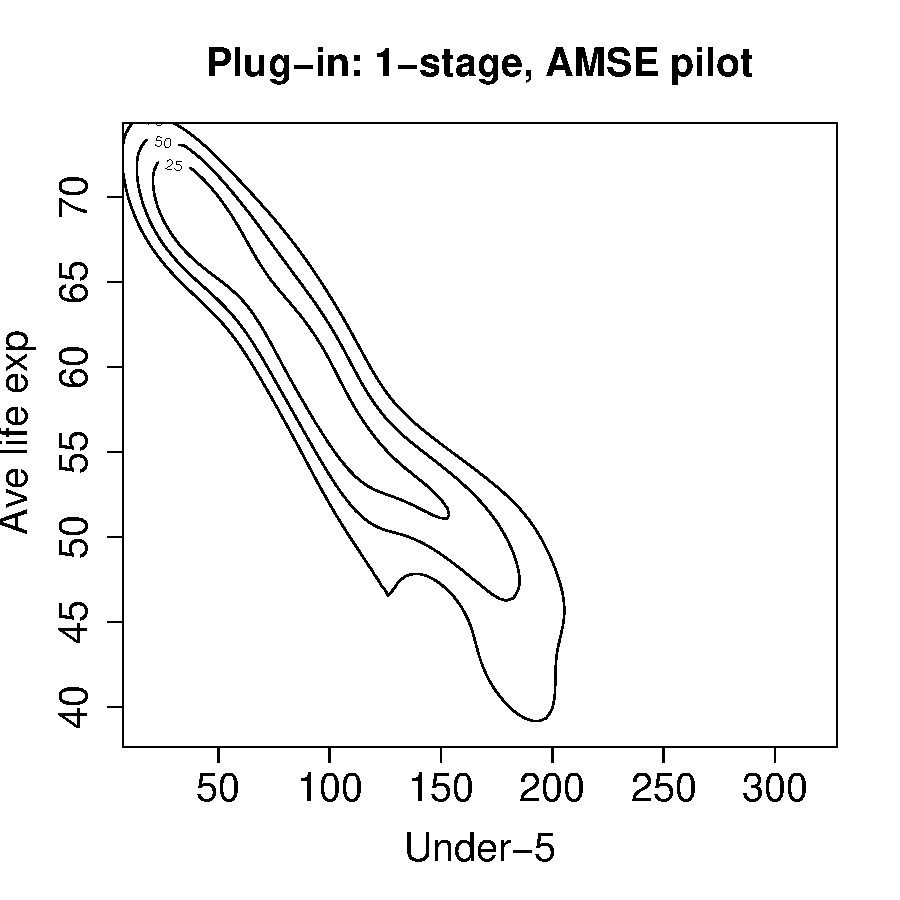
\includegraphics{kde-006}
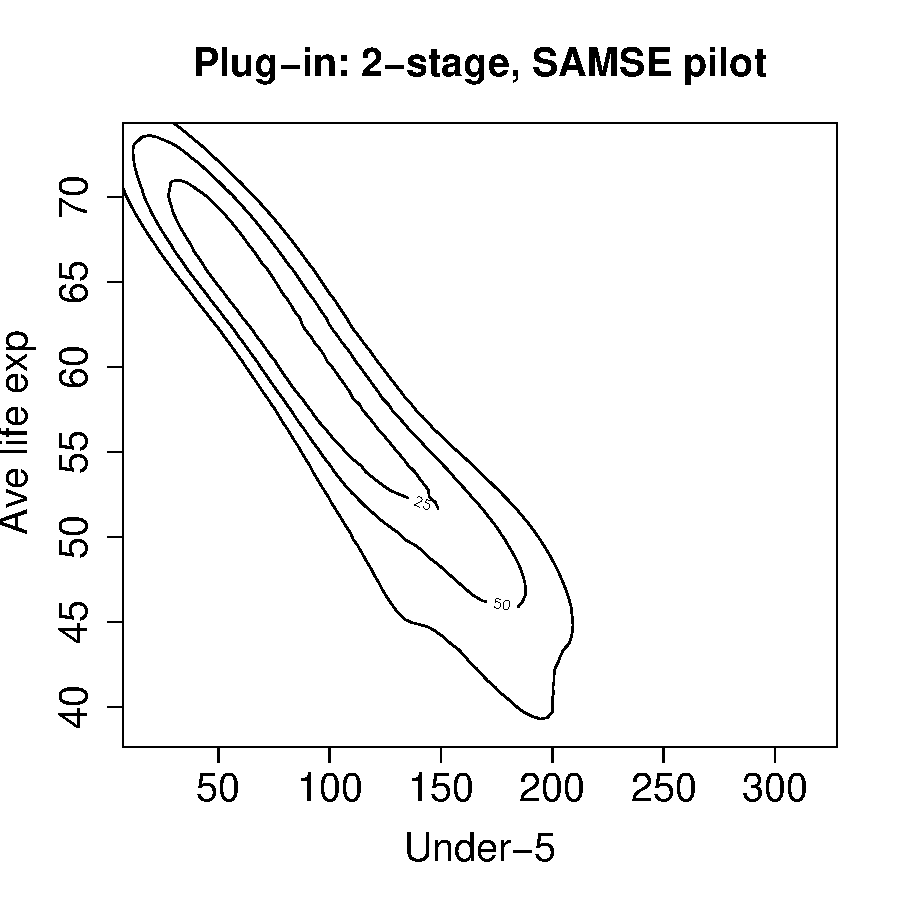
\includegraphics{kde-007}
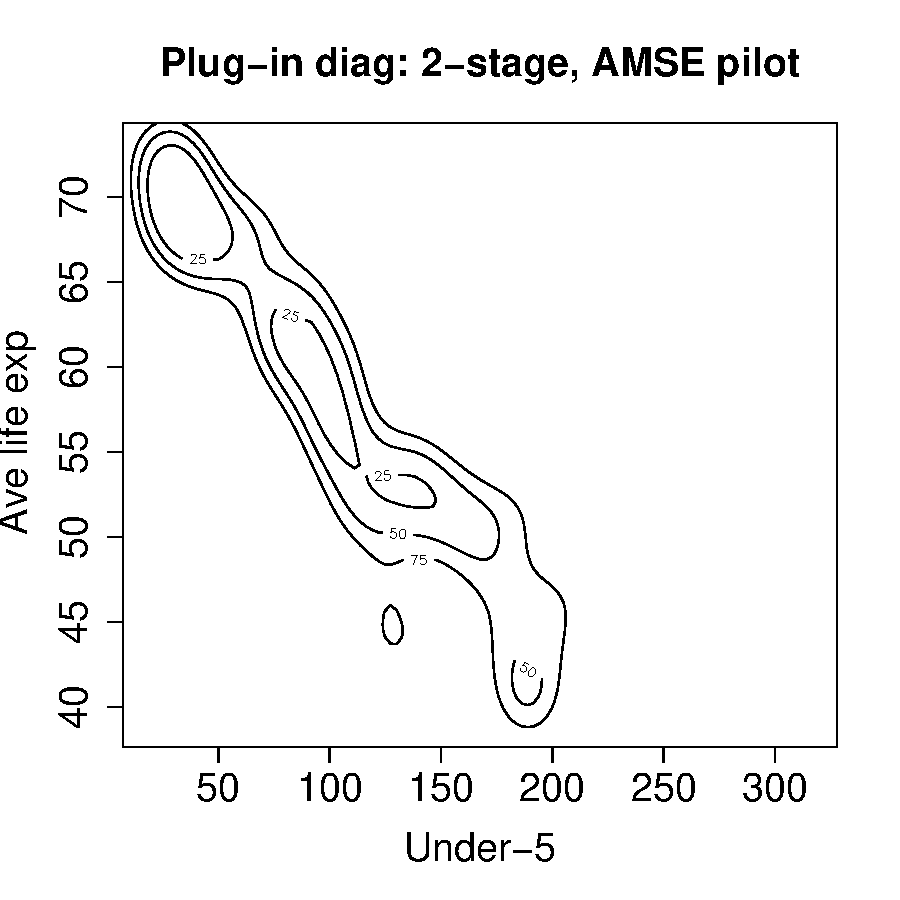
\includegraphics{kde-008}
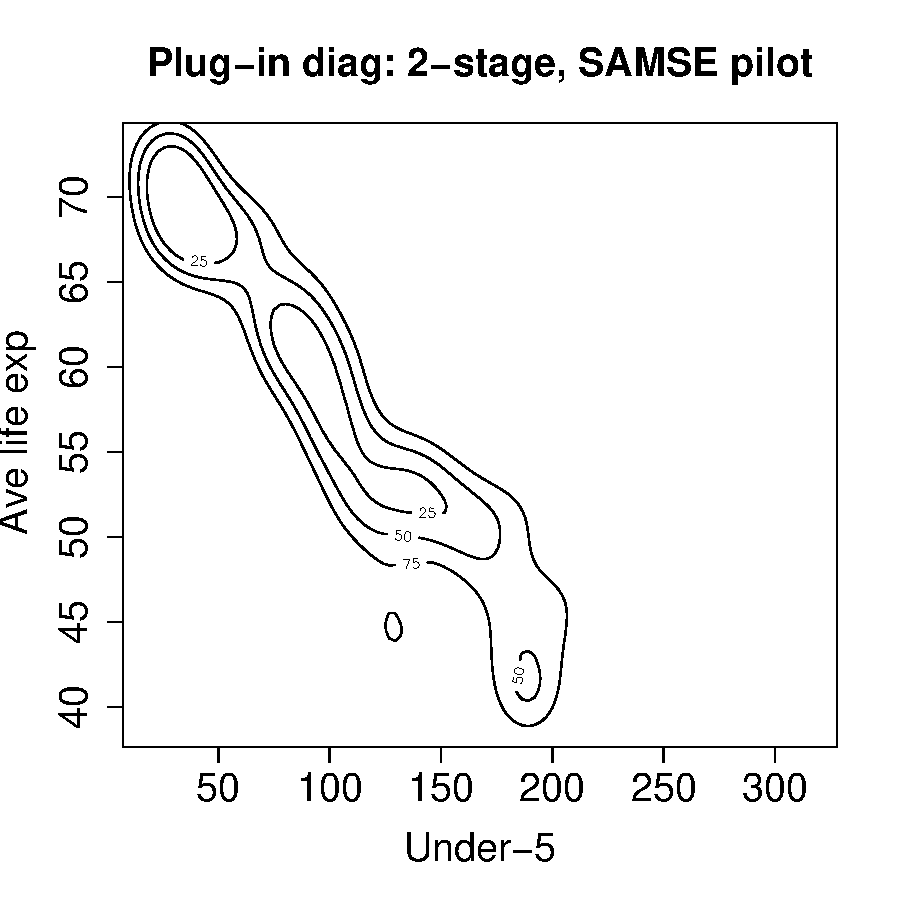
\includegraphics{kde-009}
%\caption{Kernel density estimates with plug-in selectors for unicef data}
%\label{fig:pi}
\end{center}
%\end{figure}

%\newpage

\section{Cross validation bandwidth selectors}

Cross-validation selectors are the main alternative to plug-in selectors.
There are three main types of cross-validation selectors: 
least squares, biased and smoothed. 

\subsection{Least squares cross validation}
\label{sec:lscv}
The bivariate version of 
the least squares cross validation (LSCV) criterion of
\citet*{rudemo82} and \citet*{bowman84} is 
$$\LSCV (\HH) = \intr2 \hat{f}(\vec{x}; \HH)^2 \ d \vecx - 2n^{-1} \sum_{i=1}^n 
\hat{f}_{-i} (\vec{X}_i; \HH),$$
where the leave-one-out estimator is 
$$\hat{f}_{-i} (\vec{x}; \HH) = (n-1)^{-1} 
\sum_{\jneqi}^n K_\HH (\vec{x} - \vec{X}_j).$$ 
The LSCV selector $\hat{\HH}_\LSCV$ 
is the minimiser of $\LSCV(\HH)$. We can rewrite LSCV as
\begin{align}
\label{eq:lscv2}
\LSCV(\HH) & = (4\pi)^{-1} n^{-1} |\HH|^{-1/2} + n^{-1} (n-1)^{-1} 
\sum_{i=1}^n \sum_{\jneqi}^n 
(K_{2\HH} - 2K_\HH) (\vec{X}_i - \vec{X}_j). 
\end{align}


\subsection{Biased cross validation}
Plug-in methods use a pilot bandwidth matrix $\G$ 
which is independent of $\HH$ to $\gmat{\Psi}_4$.
For BCV, we set $\G = \HH$ and use slightly different estimators.    
There are two versions of BCV, depending on the 
estimator of $\psi_{r_1, r_2}$ with $r_1 + r_2 = 4,$  see \citet*{sain94}. 
We can use
\begin{equation}
\label{eq:leave-out1}
\check{\psi}_{r_1, r_2} (\HH) =
n^{-2} \sum_{i=1}^{n}\sum_{\jneqi}^{n} 
K^{(r_1, r_2)}_{2\HH} (\vec{X}_i - \vec{X}_j)
\end{equation}
or we could use 
\begin{equation}
\label{eq:leave-out2} \tilde{\psi}_{r_1, r_2} (\HH) = n^{-1}
\sum_{i=1}^n \hat{f}_{-i}^{(r_1, r_2)} (\vec{X}_i; \HH) =
n^{-1} (n-1)^{-1} \sum_{i=1}^{n}\sum_{\jneqi}^{n} 
K^{(r_1, r_2)}_{\HH} (\vec{X}_i - \vec{X}_j).
\end{equation}
The estimates $\check{\gmat{\Psi}}_4$ and
$\tilde{\gmat{\Psi}}_4$ are obtained from $\gmat{\Psi}_4$ by substituting
$\check{\psi}_{r_1, r_2}$ and $\tilde{\psi}_{r_1, r_2}$  for $\psi_{r_1, r_2}.$
The BCV1 function is the version of BCV with $\check{\gmat{\Psi}}_4$ 
\begin{equation}
\label{eq:bcv1}
\BCV 1 (\HH) = (4\pi)^{-1}n^{-1} |\HH|^{-1/2} + \tfrac{1}{4} (\VECH^T \HH)
\check{\gmat{\Psi}}_4  (\VECH \HH)
\end{equation}
and the BCV2 function is the version with $\tilde{\gmat{\Psi}}_4$ 
\begin{equation}
\label{eq:bcv2}
\BCV 2 (\HH) =(4\pi)^{-1} n^{-1} |\HH|^{-1/2} + \tfrac{1}{4} (\VECH^T \HH)
\tilde{\gmat{\Psi}}_4  (\VECH \HH).
\end{equation}
The BCV selectors $\hat{\HH}_\BCV$ are the minimisers of the appropriate 
BCV function.

\subsection{Smoothed cross validation}
\label{sec:scv}
Smoothed cross validation (SCV), introduced by \citet*{hall92}, 
can be thought of as a hybrid of LSCV and BCV.  The SCV 
criterion takes the asymptotic integrated variance from the BCV but attempts
to estimate the integrated squared bias exactly rather than using its asymptotic
form
\begin{align}
\label{eq:scv_norm}
\SCV (\HH) &= (4\pi)^{-1} n^{-1} |\HH|^{-1/2} 
+ n^{-2} \sum_{i=1}^n
\sum_{j=1}^n (K_{2\HH + 2\G} - 2K_{\HH + 2\G} + K_{2\G})
(\vec{X}_i - \vec{X}_j). 
\end{align}
The SCV selector $\hat{\HH}_\SCV$ is the minimiser of $ \SCV(\HH).$

Again, we consider pilot bandwidth matrices of the form  $\G = g^2 \mat{I}$.
We generalise the process of \citet*{jones91b} to find an optimal 
pilot bandwidth selector.
We can show that the AMSE optimal pilot selector is
\begin{equation}
g_\AMSE = \left[ \frac{12 C_{\mu_2}}
 { (-4 C_{\mu_1} + \sqrt{C_{\mu_0}}) n }\right] ^{1/8}
\label{eq:gamse}
\end{equation}
where $C_{\mu_0}, C_{\mu_1}, C_{\mu_2}$ are constants.  The details of the derivation
of this pilot bandwidth is available in \citet*{duong05}.

\subsection{R examples}
\label{sec:pi_eg}

We continue with the \texttt{unicef} data. 
\texttt{Hlscv} and \texttt{Hlscv.diag} are the full and diagonal
LSCV selectors. (The \texttt{Hstart} argument in the below code specifies the initial
value for the numerical minimisation - it can be specified
for any of the bandwidth selector functions). 
\texttt{Hbcv} implements both BCV1 and BCV2. The
default is BCV1; set \texttt{whichbcv=2} to use BCV2.
Their diagonal counterpart is \texttt{Hbcv.diag}. 
\texttt{Hscv} is the full SCV selector (no diagonal version is available).
Its argument \texttt{pre} is the same as for \texttt{Hpi} and \texttt{Hpi.diag}
in Section \ref{sec:pi_eg}.  
\begin{Schunk}
\begin{Sinput}
> Hlscv1 <- Hlscv(unicef)
\end{Sinput}
\begin{Soutput}
          [,1]      [,2]
[1,] 388.18250 -83.34084
[2,] -83.34084  25.12909
\end{Soutput}
\begin{Sinput}
> Hlscv2 <- Hlscv.diag(unicef, Hstart = Hlscv1)
\end{Sinput}
\begin{Soutput}
         [,1]     [,2]
[1,] 194.4292  0.00000
[2,]   0.0000 11.11751
\end{Soutput}
\begin{Sinput}
> Hbcv1 <- Hbcv(unicef)
\end{Sinput}
\begin{Soutput}
          [,1]      [,2]
[1,] 1087.0682 135.33067
[2,]  135.3307  23.58613
\end{Soutput}
\begin{Sinput}
> Hbcv2 <- Hbcv.diag(unicef, whichbcv = 2)
\end{Sinput}
\begin{Soutput}
         [,1]     [,2]
[1,] 1072.781 0.000000
[2,]    0.000 9.298466
\end{Soutput}
\begin{Sinput}
> Hscv1 <- Hscv(unicef, pre = "sphere")
\end{Sinput}
\begin{Soutput}
          [,1]      [,2]
[1,] 1323.3189 -191.9278
[2,] -191.9278   35.0105
\end{Soutput}
\begin{Sinput}
> Hscv2 <- Hscv(unicef, pre = "scale")
\end{Sinput}
\begin{Soutput}
          [,1]      [,2]
[1,] 694.14462 -73.09935
[2,] -73.09935  17.49451
\end{Soutput}
\end{Schunk}
\begin{Schunk}
\begin{Sinput}
> fhat1 <- kde(unicef, Hlscv1)
> fhat2 <- kde(unicef, Hlscv2)
> fhat3 <- kde(unicef, Hbcv1)
> fhat4 <- kde(unicef, Hscv1)
\end{Sinput}
\end{Schunk}
\begin{Schunk}
\begin{Sinput}
> plot(fhat1, main = "LSCV")
> plot(fhat2, main = "LSCV diag")
> plot(fhat3, main = "BCV")
> plot(fhat4, main = "SCV")
\end{Sinput}
\end{Schunk}
\begin{center}
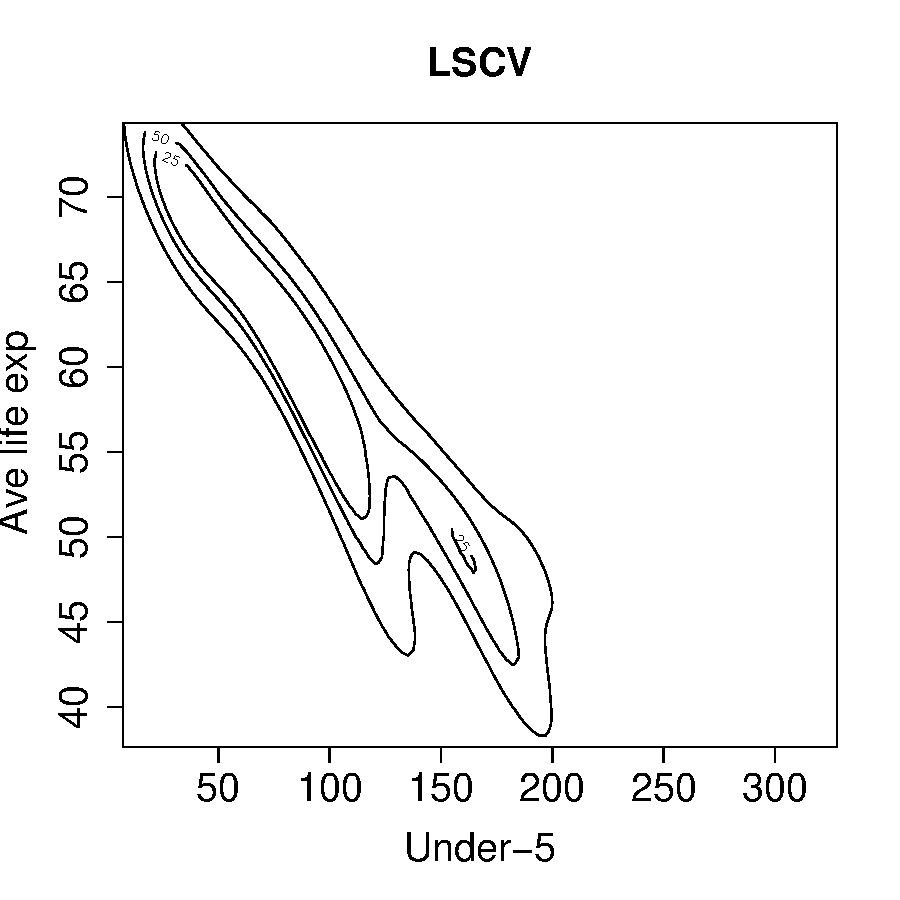
\includegraphics{kde-014}
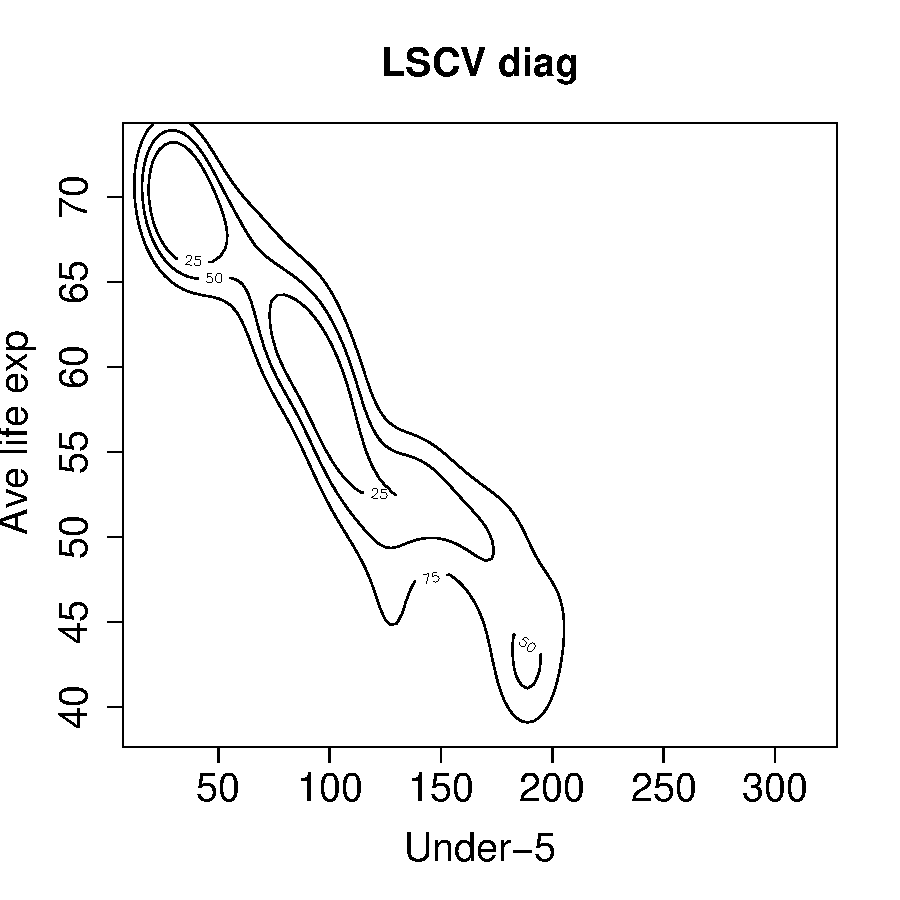
\includegraphics{kde-015}
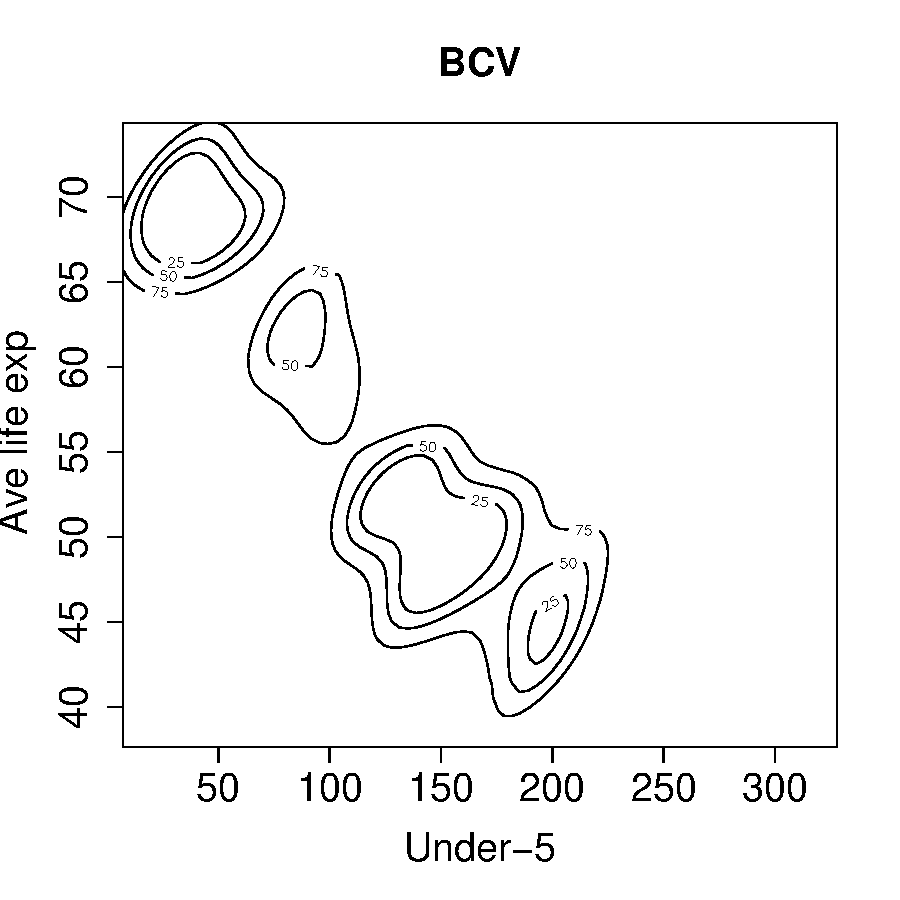
\includegraphics{kde-016}
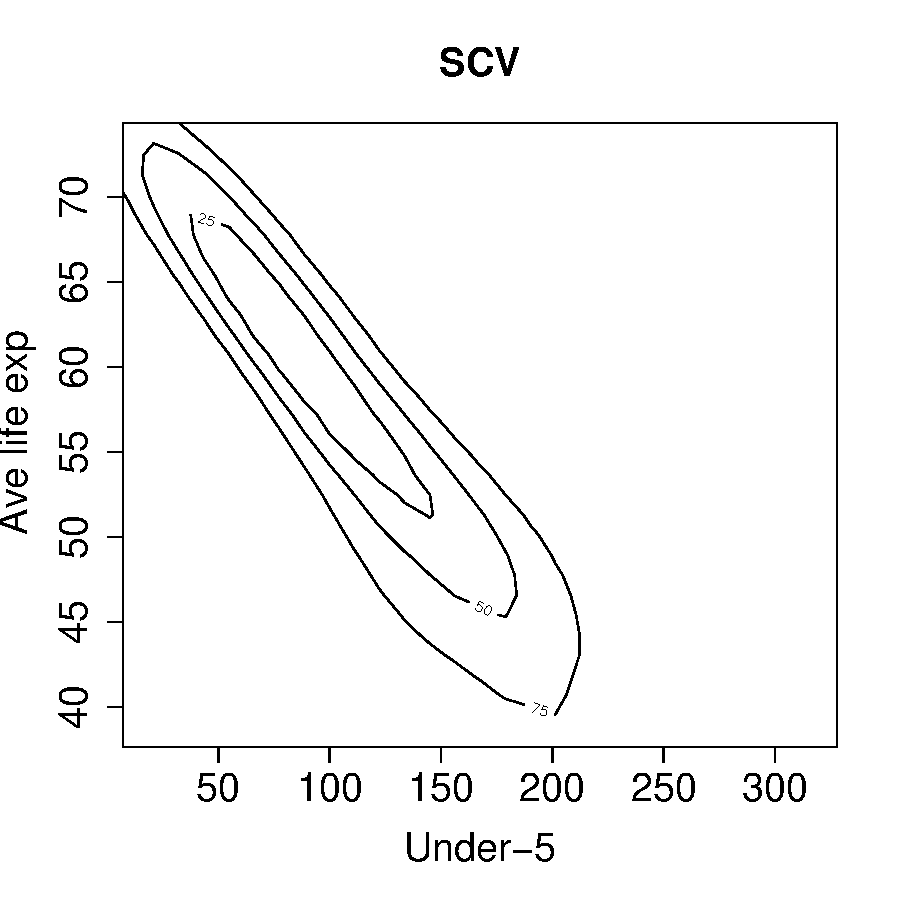
\includegraphics{kde-017}
\end{center}

%\caption{Cross validation selectors for unicef data}
%\label{fig:cv}

%\end{figure}

\section{More graphics}
There are many options with plotting kernel density estimates. 
%as illustrated in Figure \ref{fig:kde}.
Slice or contour plots are the default or can be explicitly called by setting
\texttt{display="slice"}. The way the contours are plotted is controlled by
\texttt{cont} or \texttt{ncont}: only one of these needs to be set. 
The argument 
\texttt{cont} takes a vector of percentages and produces a set of contours
at the levels corresponding to the percentages of the maximum height of the 
density estimate. The argument 
\texttt{ncont} takes a number and \texttt{R} tries to 
compute a pretty set of \texttt{ncont} contours.  
The colour(s) of the contour lines is \texttt{lcol} and
the colour(s) of the plotting symbols is \texttt{ptcol}.
The logical flags \texttt{drawlabels} and \texttt{drawpoints} indicate
whether to draw the labels for the contours levels or the data points.

An alternative to contour plots are the image or heat plots,
called by \texttt{display="image"}.  These 
are similar to contour plots except that the heights of the density 
estimate are represented by different colours rather than with
different level curves. The default colours is \texttt{heat.colors}
but we use instead \texttt{rev(heat.colors)} which gives us the high 
values as red and the low values (close to zero) as white with
yellow/orange as intermediate. 

The other alternative is a perspective or wire-frame plot, 
called by \texttt{display="persp"}. This is an attempt
to capture the three-dimensional structure more directly than the 
image or contour plots.

%\begin{figure}[!htp]

\begin{Schunk}
\begin{Sinput}
> plot(fhat4, lcol = "blue", ptcol = "black", cont = seq(10, 90, 
+     by = 20))
> plot(fhat4, ncont = 8, drawlabels = FALSE, drawpoints = FALSE)
> plot(fhat4, display = "image", col = rev(heat.colors(100)))
> plot(fhat4, display = "persp")
\end{Sinput}
\end{Schunk}
\begin{center}
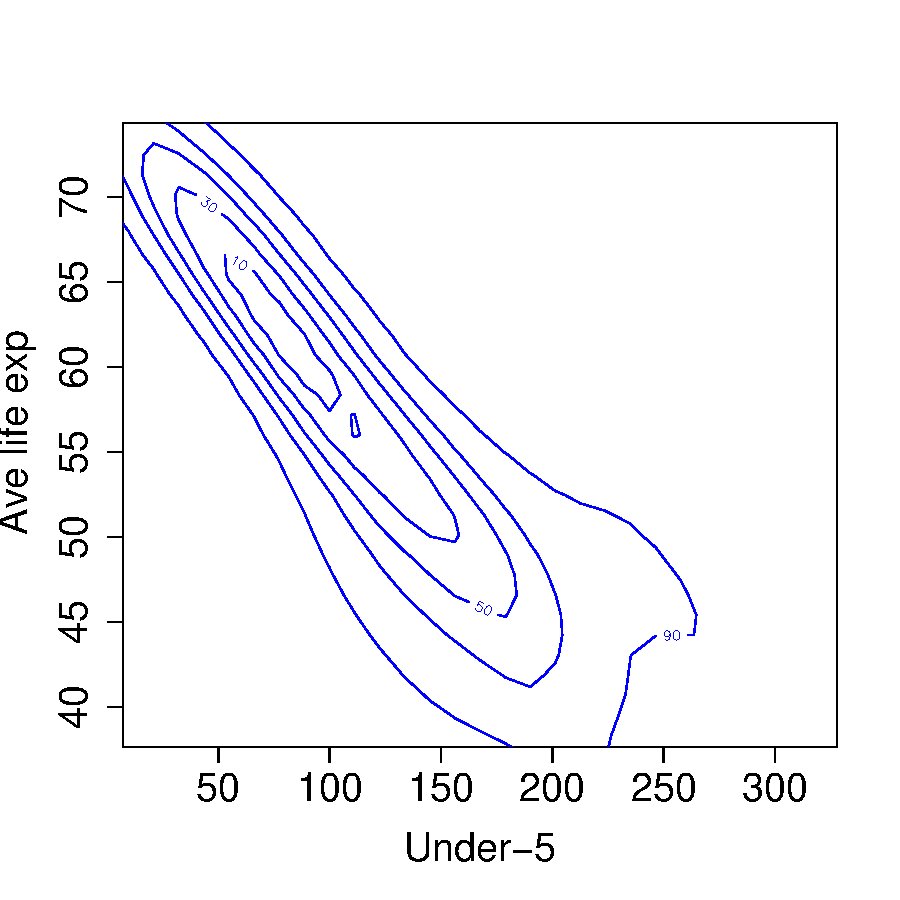
\includegraphics{kde-019}
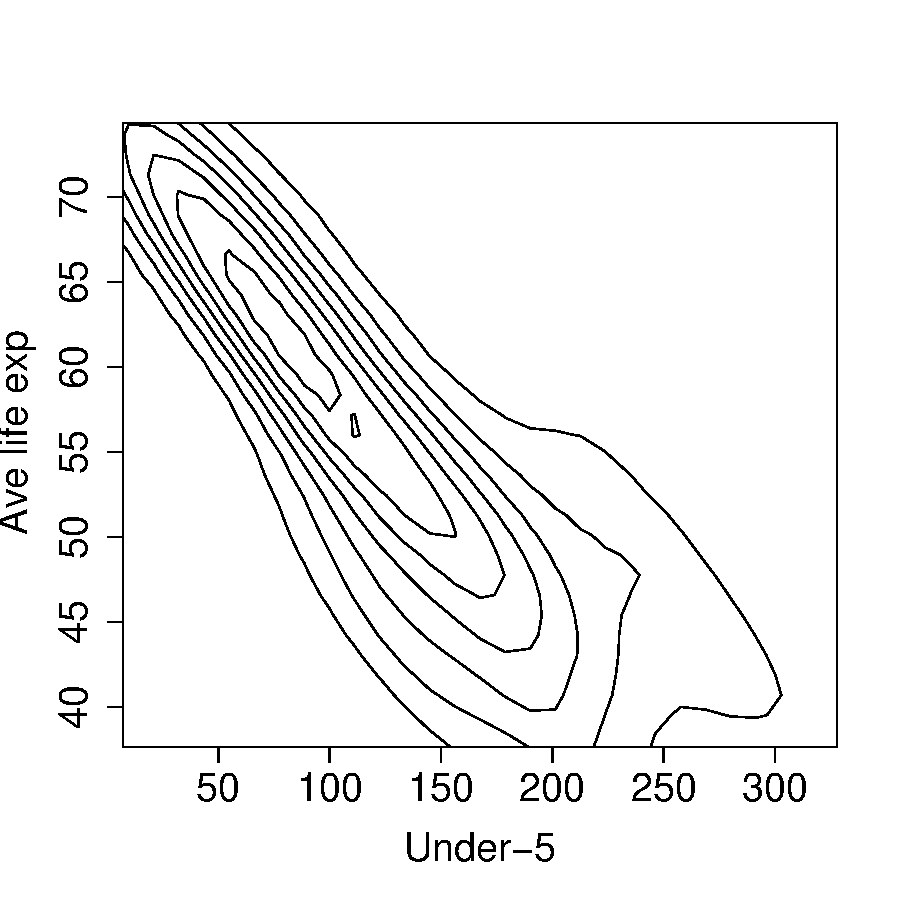
\includegraphics{kde-020}
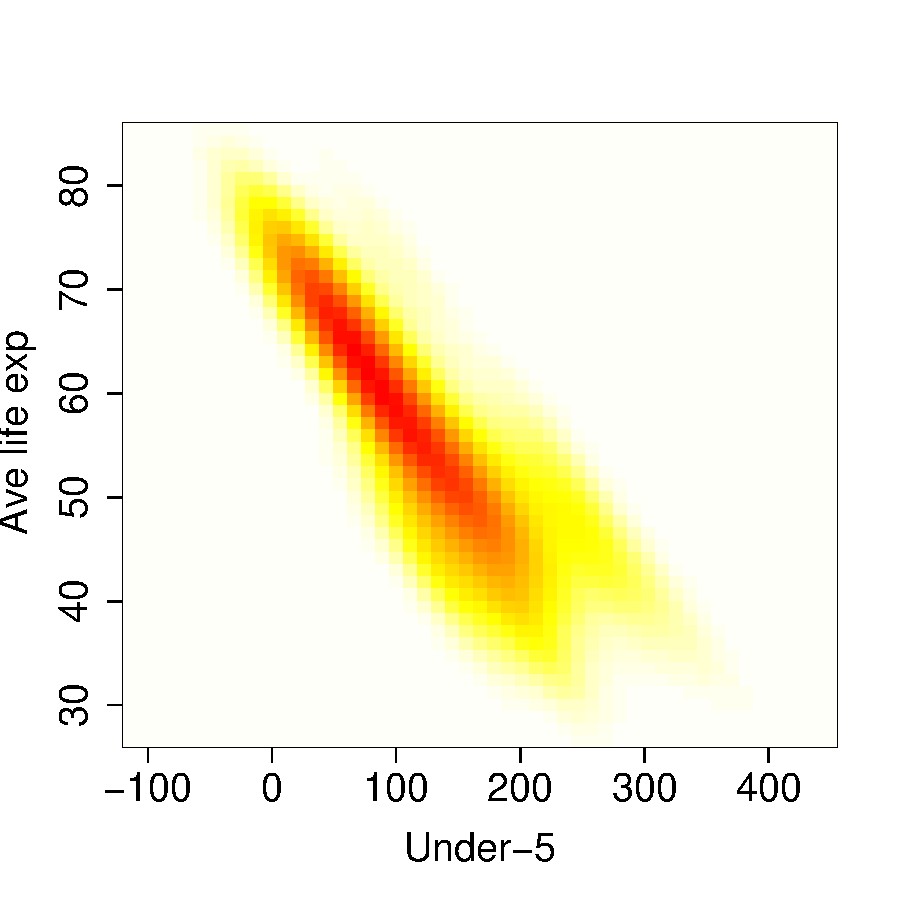
\includegraphics{kde-021}
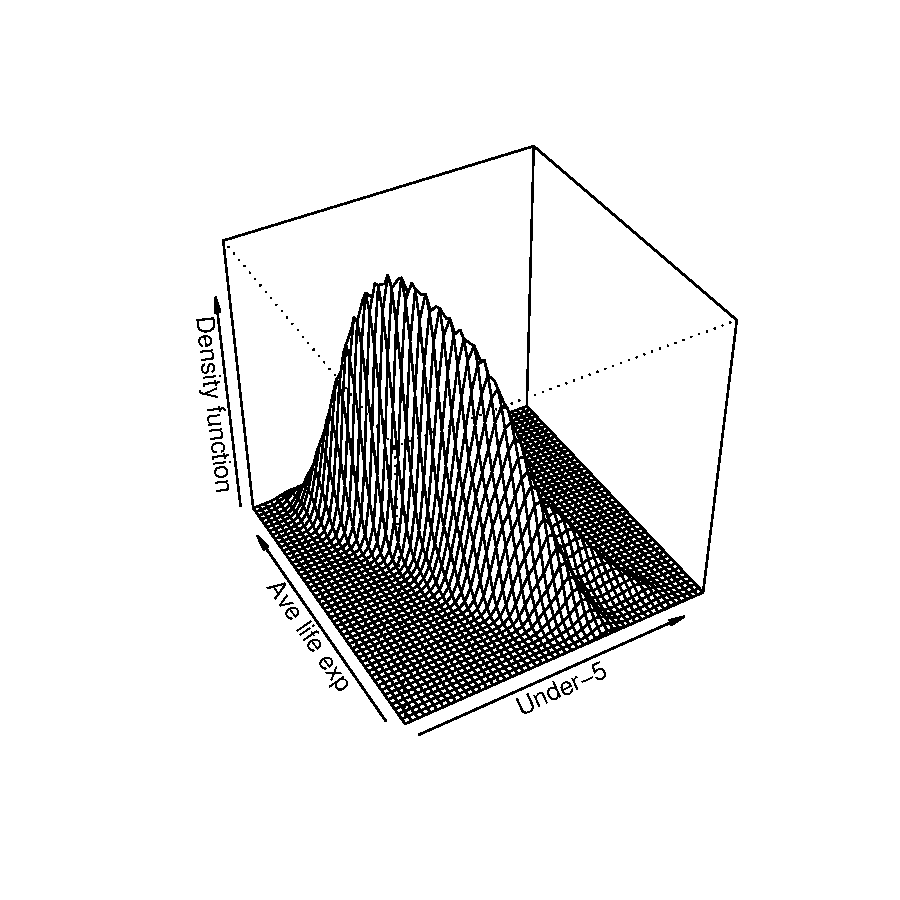
\includegraphics{kde-022}
%\caption{Graphics options for KDE plots}
%\label{fig:kde} 
\end{center}
%\end{figure}


\section{Large sample sizes and binned kernel estimation}
\label{sec:binned}

For large sample sizes, direct computation of kernel estimates becomes 
computationally difficult. One common technique for increasing computational
speed for these large samples is binned kernel estimation, 
see \citet*[Appendix~D]{wand94}. Unfortunately binned estimation is only defined 
with diagonal bandwidth matrices. So appilcable cases include 
computing the pilot bandwidth matrices
(which are parameterised as $g^2 \mat{I}$) for general plug-in and SCV selectors;
and for kernel density estimators with diagonal bandwidth matrices. 


\begin{Schunk}
\begin{Sinput}
> mus <- rbind(c(-2, 2), c(0, 0), c(2, -2))
> Sigmas <- rbind(diag(2), 0.8 * invvech(c(1, -0.9, 1)), diag(2))
> cwt <- 3/11
> props <- c((1 - cwt)/2, cwt, (1 - cwt)/2)
> plotmixt(mus, Sigmas, props, display = "image", col = rev(heat.colors(100)))
> x <- rmvnorm.mixt(10000, mus, Sigmas, props)
> H.pidiag <- Hpi.diag(x, binned = TRUE)
> H.pi <- Hpi(x, binned = TRUE)
\end{Sinput}
\end{Schunk}
For large sample sizes, we don't recommend plotting with slice/contour plots
because computing the relative contour heights is computationally intensive.
Instead, image or perspective plots are more efficient.
\begin{Schunk}
\begin{Sinput}
> fhat.diag <- kde(x, H = H.pidiag, binned = TRUE)
> plot(fhat.diag, display = "image", col = rev(heat.colors(100)))
\end{Sinput}
\end{Schunk}
\begin{center}
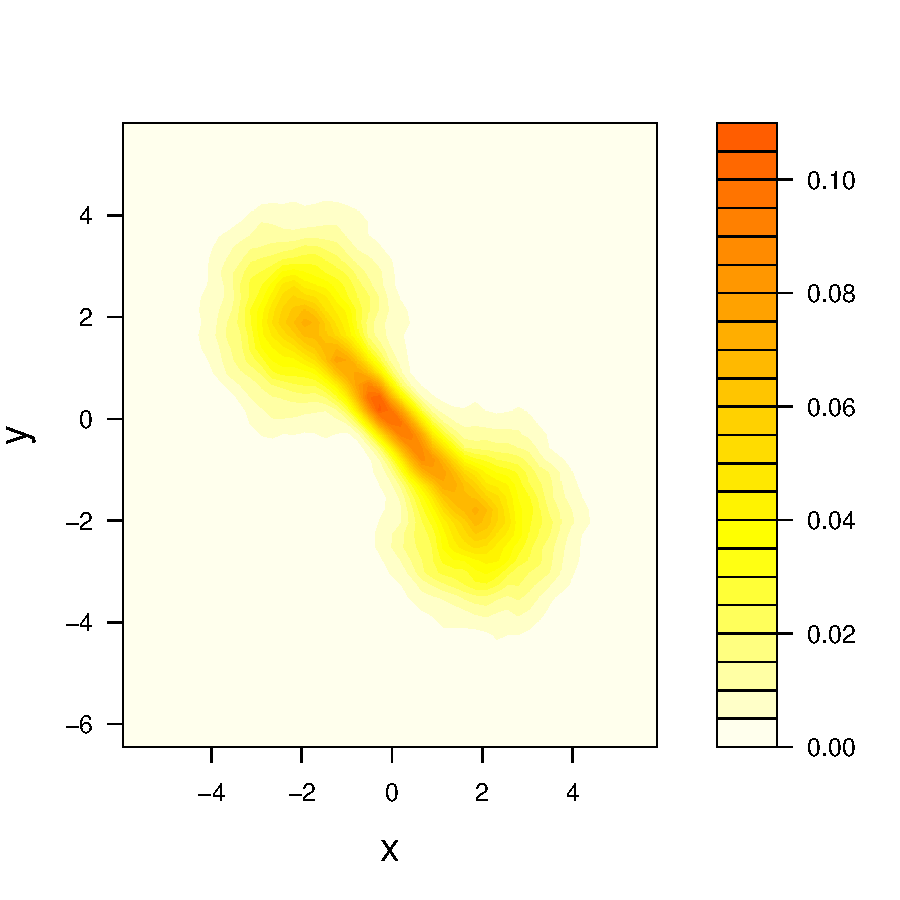
\includegraphics{kde-025}
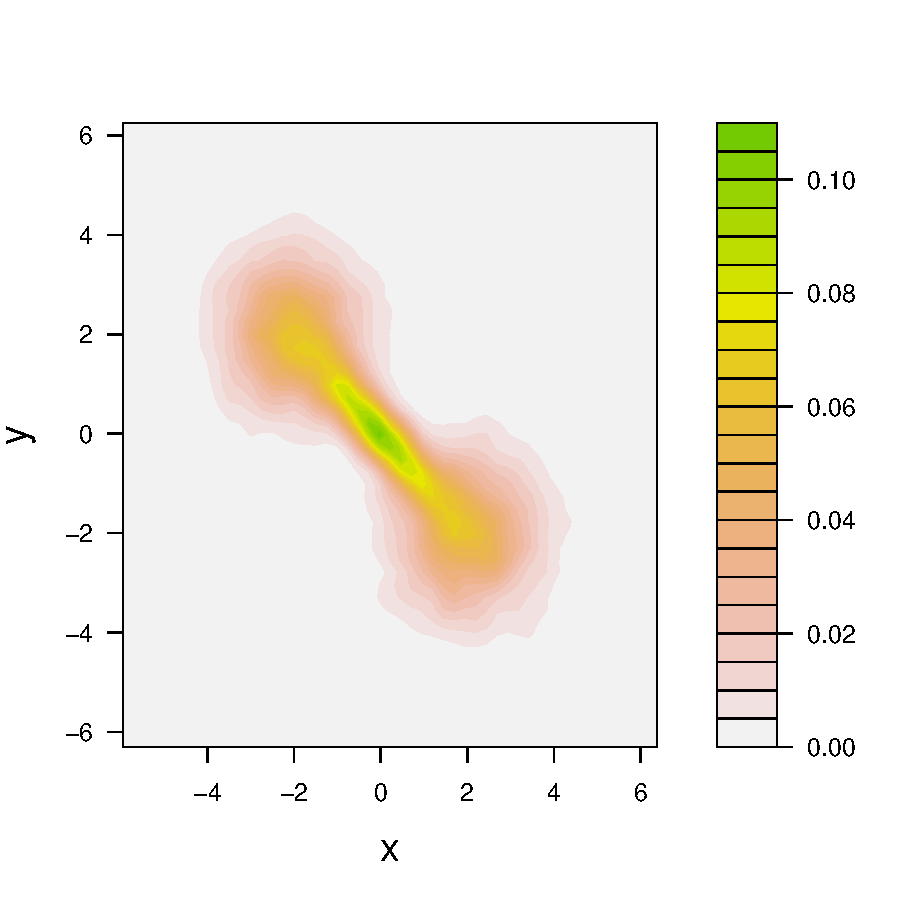
\includegraphics{kde-026}
\end{center}

%fhat <- kde(x, H=H.pi)
%plot(fhat, display="image", col=rev(heat.colors(100)))
%fhat <- kde(x, H=H.pi, gridsize=rep(51,2))
%plot(fhat, display="image", col=rev(heat.colors(100)), cex.lab=1.6, cex.axis=1.6) 

\section{Pre-transformations}
\label{sec:pre}
The plug-in and SCV selector functions use pilot bandwidths of the 
form $\mat{G} = g^2 \mat{I}$ which will be 
inappropriate if the dispersion of the data differs 
markedly between the two coordinate 
directions. We estimate using the transformed data 
$\vec{X}_1^*, \vec{X}_2^*, 
\dots, \vec{X}_n^*$, where the transformation is either {\em sphering} 
$$\vec{X}^*= \mat{S}^{-1/2} \vec{X}$$
where $\mat{S}$ is the sample covariance matrix of the untransformed data; 
or {\em scaling}
$$\vec{X}^*= \mat{S}_D^{-1/2} \vec{X}$$
where $\mat{S}_D = {\rm diag}(s_{1}^2, s_{2}^2)$ and $s_1^2, s_2^2$ are 
the marginal sample variances. The  
bandwidth matrix $\hat{\HH}^*$
for the sphered or scaled data can be back transformed to the original scale by 
$\hat{\HH} = \mat{S}^{1/2} \hat{\HH}^* \mat{S}^{1/2}$ or 
$\hat{\HH} = 
\mat{S}_D^{1/2} \hat{\HH}^* \mat{S}_D^{1/2}$, as appropriate.


\section{General recommendations}

It is generally advisable to try a few 
different selectors and visually examine the resulting density estimates. 
One of the primary motivations for the author to write the \ks \ package 
is to make visualising kernel density estimates easy.
There are many different bandwidth selectors available in \ks: they may
now pose a problem of \emph{too} much choice.
The full bandwidth selectors will be better than their diagonal counterparts
when the data have large mass oriented obliquely to the co-ordinate axes 
(as is the case for the \texttt{unicef} data). 
Amongst the full selectors, we advise against using the BCV selector. 
The LSCV selector is useful in some cases though its performance is 
known to be highly variable. The 2-stage plug-in and the SCV selectors
can be viewed as generally recommended bandwidth selectors.



\bibliographystyle{apalike} %%apsrmp or apalike
%\bibliography{/c/tduong/home/research/references}

\begin{thebibliography}{}
\bibitem[Bowman, 1984]{bowman84}
Bowman, A.~W. (1984).
\newblock An alternative method of cross-validation for the smoothing of
  density estimates.
\newblock {\em Biometrika}, \textbf{71}, 353--360.

\bibitem[Duong and Hazelton, 2003]{duong03}
Duong, T. and Hazelton, M.~L. (2003).
\newblock Plug-in bandwidth matrices for bivariate kernel density estimation.
\newblock {\em Journal of Nonparametric Statistics}, \textbf{15}, 17--30.

\bibitem[Duong and Hazelton, 2005]{duong05}
Duong, T. and Hazelton, M.~L. (2005).
\newblock Cross-validation bandwidth matrices for multivariate kernel density
  estimation.
\newblock {\em Scandinavian Journal of Statistics}, \textbf{32}, 485--506.

\bibitem[Hall et~al., 1992]{hall92}
Hall, P., Marron, J.~S., and Park, B.~U. (1992).
\newblock Smoothed cross-validation.
\newblock {\em Probability Theory and Related Fields}, \textbf{92}, 1--20.

\bibitem[Jones et~al., 1991]{jones91b}
Jones, M.~C., Marron, J.~S., and Park, B.~U. (1991).
\newblock A simple root $n$ bandwidth selector.
\newblock {\em The Annals of Statistics}, \textbf{19}, 1919--1932.

\bibitem[Rudemo, 1982]{rudemo82}
Rudemo, M. (1982).
\newblock Empirical choice of histograms and kernel density estimators.
\newblock {\em Scandinavian Journal of Statistics. Theory and Applications},
  \textbf{9}, 65--78.

\bibitem[Sain et~al., 1994]{sain94}
Sain, S.~R., Baggerly, K.~A., and Scott, D.~W. (1994).
\newblock Cross-validation of multivariate densities.
\newblock {\em Journal of the American Statistical Association}, \textbf{89}, 807--817.

\bibitem[Sheather and Jones, 1991]{sheather91}
Sheather, S.~J. and Jones, M.~C. (1991).
\newblock A reliable data-based bandwidth selection method for kernel density
  estimation.
\newblock {\em Journal of the Royal Statistical Society. Series B.
  Methodological}, \textbf{53}, 683--690.

\bibitem[Simonoff, 1996]{simonoff96}
Simonoff, J.~S. (1996).
\newblock {\em Smoothing Methods in Statistics}.
\newblock Springer-Verlag, New York.

\bibitem[Wand and Jones, 1994]{wand94}
Wand, M.~P. and Jones, M.~C. (1994).
\newblock Multivariate plug-in bandwidth selection.
\newblock {\em Computational Statistics}, \textbf{9}, 97--116.

\end{thebibliography}

\end{document}
